%----------------------------------------------------------------------------
%\chapter{\Kubernetes}
%\label{sec:Kubernetes}
%----------------------------------------------------------------------------
\chapter{Irodalomkutatás}
\label{sec:Publications}
A félév során több publikációt is elolvastam, hogy tisztább legyen a kutatási terület. A következőben szeretném összefoglalni, hogy eddig milyen irányban történtek haladások.

Több oldalról meg lehet fogni a skálázás és szorosan hozzá köthető erőforrás elosztás területét. Minden kutatás kicsit más szempontból vizsgálja, más áll a középpontban.

A legátfogóbb ismertető a témában \emph{Cloud resource management: A survey on forecasting and profiling models}\citep{CloudResourceManagement} című cikk. Szépen összegzi a téma megjelenésekor ismert kutatásokat és rendszerezi azokat. Strukturáltan összegyűjtötték, hogyan és miért lehet szükséges az egyes alkalmazások profilozása, milyen akadályokkal szembesülhetünk.

Az alkalmazás mélyebb megismerésével lehetőségünk van előrejelzéseket adni a viselkedésére és ezáltal az erőforrás felhasználást is ügyesebben kezelni. Kritizálják, hogy a legtöbb kutatás elég szűk területet érint és nagyon specifikus kérdéskört vizsgál, miközben figyelmen kívül hagyja a felhős környezet változékonyságát és a valóságnál statikusabb rendszerként vannak kezelve. 

Ötleteket is tudunk meríteni, hogy milyen értékeke érdemes a mérések során figyelembe venni.
Példaként említi  a processzor, memória, I/O lemez késleltetések, válaszidő, áteresztő képesség
mérését. Utóbbi kettő rendszeresen előfordul a szolgáltatási szint megállapodásokban (SLA), ami a felhasználó által érzékelhető szolgáltatási szint (QoE) alapjának is tekinthető. 
Ezek a tulajdonságok vannak összefoglalva a \ref{fig:applicationprofiling} ábrán, ami szintén a cikkben jelent meg.

Gyakran elfelejtődik, de a cikkben hangsúlyozva van, hogy a rendszer monitorozása, döntéshozás és közbeavatkozás önmagukban is jelentenek valamekkora plusz költséget. \\


% Alkalmazás profilozás mind-map ---------------------------------------------
\begin{figure}[!ht]
\centering
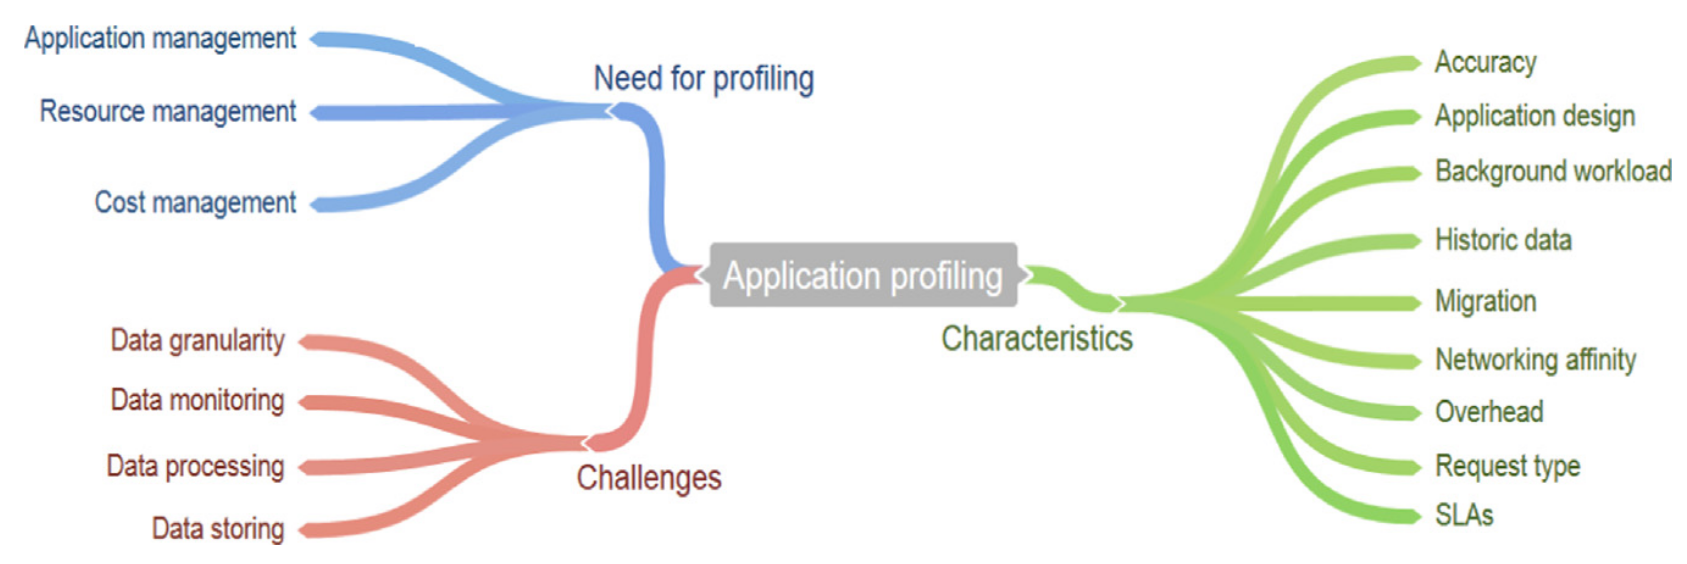
\includegraphics[width=150mm, keepaspectratio]{figures/applicationprofiling.png}
\caption{Alkalmazás profilozás elmetérképe\citep{CloudResourceManagement}}
\label{fig:applicationprofiling}
\end{figure}

Korábban már a tanszéken is foglalkoztak Kubernetesben történő skálázással. Az \emph{Adaptive scaling of Kubernetes pods}\cite{AdaptiveScalingOfPods} címen megjelent kutatás keretén belül sikeresen implementáltak egy automatikus skálázót, ami képes kihasználni a vertikális és horizontális skálázásban rejlő előnyöket. Az algoritmus első részében megkeresi az egy pod számára ideális erőforrás-használatot, ami tekinthető a vertikális skálázásnak. Később pedig az így megtalált konfigurációval történik az alkalmazás horizontális skálázása. Ez a megvalósítás egybeesik a korábbi kutatás következtetésével\citep{bscThesis}, mely szerint általában jobb eredményt kapunk VPA segítségével, azonban feltehetően minden esetben létezik egy felső határ, ami után már nem kapunk jobb kiszolgálási eredményeket. 

A diplomaterv későbbi részében érdekes eredményeket kaphatunk, ha összehasonlítjuk ezt a megoldást a Kubernetes alapértelmezett skálázásával egy komplexebb szolgáltatásháló esetén.

Több cikk\cite{AdaptiveScalingOfPods}\citep{PredictingUsageAndProactiveScaling} is említést tesz
arról, hogy a jelenlegi módszertan alapján nehéz eltalálni az optimális erőforrás értékeket és ezzel
együtt a skálázást. Ez főként onnan jön, hogy jelenleg a skálázók kevés logikával és metrikával
működnek, ezért indításukkor, kézzel kell megadni a szükséges értékeket. Ez igaz az erőforrás
felhasználásra is. Ebben az esetben is az alkalmazás üzemeltetőja adja meg indítás idejében a
paramétereket, amik befolyásolják a kiszolgálás minőségét is. 

Érdekes kérdés, ami irodalomkutatás során fogalmazódott meg, hogy a skálázó minél optimálisabb döntéséhez minél több adatra van szükség. Ez bizonyos alkalmazási területek körében problémás lehet. Hogyha az alkalmazás tulajdonosa nem szeretné, hogy megfigyeljék, hogy milyen egyéb szolgáltatásokkal van kapcsolatban, mennyi lekérdezés, felhasználó használja, milyen arányban oszlik meg a terhelés a rendszere egységei között, akkor a végső döntés is kevesebb információ ismerete alapján lesz meghozva. Érdekes kérdéskör ez is, hogy hol van a határa a személyes adatoknak és mennyire lehet ezeket figyelembe venni az optimálisabb erőforrás elosztáshoz.

Több megoldás bontakozott ki a tanulmányozott cikkekből. Vannak olyan megoldások, amik a rendszert fehér dobozként kezelik, amiben minden paraméter kiolvasható és befolyásolható, míg vannak olyanok, amik feketedobozként modellezik az alkalmazásokat és a belső működésük számunkra teljesen fedett.\citep{TowardsAnAdaptive}. Az első esetben van lehetőségünk analitikus modelleket gyártani és ezeket alapul véve jósolni, javaslatokat tenni. Utóbbi esetben, jó kiindulási alap lehetnek a gépi tanulásos modellek. Itt megjegyezhető, hogy számontarthatjuk a modellünk bizonyos paraméterek melletti bizonytalanságát mint tényezőt és ezeken helyeken több mérést végezve javítható a modell bizonyossága\citep{TowardsAnAdaptive}.

Elterjedt kutatási terület, hogyan lehet ilyen jellegű feladatok megoldásában segítségül hívni a neurális-hálózatokat, illetve egyéb gépi-tanulásos modelleket. Ilyen modell lehet például a Markov-láncok, ami képesek a valós rendszerekben megfigyelhető periodicitásokat figyelembe venni\citep{CloudScale}. Ilyen ismétlődés több nagyságrendben is elképzelhető, például egy napon belül is létezik, de létezhet nagyobb távlatban, például az évszakkal összefüggően is\citep{PredictingUsageAndProactiveScaling}.




